\section{Discusión de Limitaciones}
A pesar del rendimiento cuantitativo y cualitativo superior demostrado por el modelo adaptado con transferencia de aprendizaje, el sistema dista de ser infalible. Identificar y comprender de manera crítica los límites operativos y los fallos sistemáticos del modelo es una etapa imperativa para robustecer su funcionamiento antes de cualquier despliegue práctico en inspecciones industriales.

\subsection{Análisis Cualitativo de Errores y Modos de Fallo}
Para profundizar en las debilidades del clasificador ResNet-50, se extrajeron 5 imágenes de validación en las cuales la red realizó predicciones erróneas. El análisis de estas muestras permitió estructurar cinco hipótesis clave sobre los modos de fallo físicos y geométricos:

\begin{enumerate}
    \item \textbf{Texturas Ambiguas y Suciedad (Falsos Positivos):} Neumáticos sanos con manchas de barro seco, piedrecillas incrustadas o reflejos de agua en la superficie son clasificados erróneamente como dañados. Los patrones lineales que forman estos elementos externos imitan el contraste de las grietas.
    \item \textbf{Sombras Proyectadas y Luz Direccional (Falsos Positivos):} Cuando las imágenes presentan una luz lateral fuerte, los surcos normales de la banda de rodadura proyectan sombras duras de gran contraste, generando bordes artificiales que el extractor convolucional confunde con grietas o roturas estructurales.
    \item \textbf{Fronteras de Daño Muy Sutiles (Falsos Negativos):} Llantas que presentan microfisuras iniciales muy finas o desgastes localizados sumamente sutiles son etiquetadas como normales por el modelo. Esto responde a la naturaleza conservadora del clasificador actual ante umbrales de probabilidad cercanos a la frontera de decisión.
    \item \textbf{Ruido en el Etiquetado del Dataset (Errores de Validación):} Se identificaron imágenes en el dataset con etiquetas erróneas de origen (por ejemplo, llantas dañadas anotadas como normales). Esto introduce un falso error de predicción en el cálculo de las métricas durante la validación del modelo.
    \item \textbf{Pérdida de Foco y Desenfoque Óptico (Falsos Negativos):} Las imágenes capturadas con ligeros movimientos de cámara o fuera del plano focal sufren de desenfoque. Al suavizarse los bordes de alta frecuencia, las primeras capas convolucionales pierden los detalles finos de la textura del caucho, causando que la red sea incapaz de identificar anomalías estrechas.
\end{enumerate}

\begin{figure}[htbp]
    \centering
    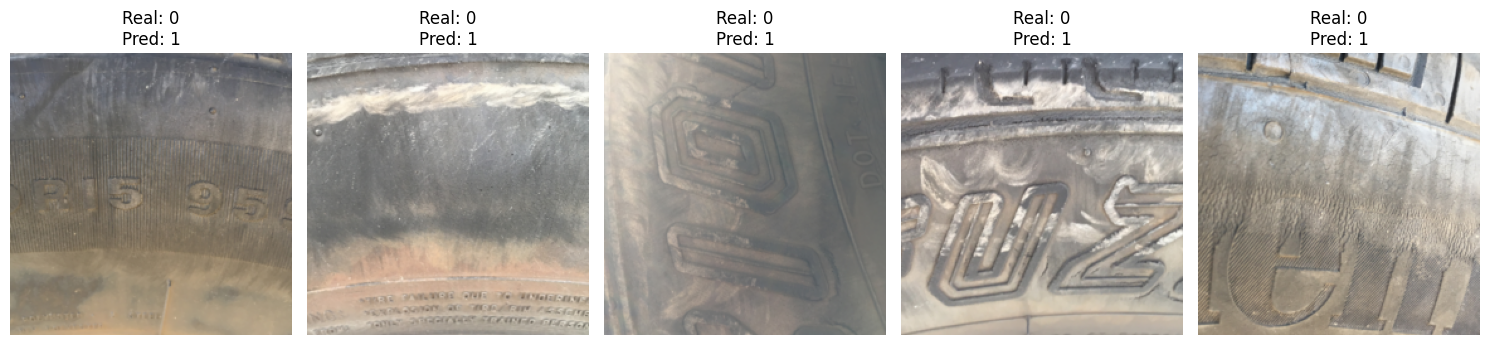
\includegraphics[width=0.9\textwidth]{Imagenes/analisis_fallos.png}
    \caption{Casos representativos de error del modelo ResNet-50 durante la validación (Etiqueta real vs Predicción).}
    \label{fig:fallos}
\end{figure}

\subsection{Conclusiones}
Este trabajo demuestra la viabilidad técnica de clasificar de forma automatizada texturas de neumáticos mediante arquitecturas convolucionales y aprendizaje por transferencia. Se concluye que:
\begin{itemize}
    \item El desbalance de datos debe ser mitigado mediante estrategias complementarias a nivel de datos (\texttt{WeightedRandomSampler}) y de pérdida (\texttt{Focal Loss}) para evitar que el gradiente ignore la clase minoritaria dañada.
    \item La transferencia de aprendizaje con ResNet-50 es significativamente superior (77.85\% exactitud y 0.8928 AUC-ROC en la versión con Focal Loss, y hasta 79.69\% de exactitud con la pérdida BCE) al entrenamiento desde cero de arquitecturas convolucionales simples, requiriendo además menor número de épocas de optimización.
    \item La interpretabilidad visual obtenida con Grad-CAM resulta indispensable para verificar que el clasificador enfoca su atención de forma justificada en los patrones texturales reales de desgaste y grietas físicas.
    \item Las limitaciones del sistema residen principalmente en la sensibilidad a variaciones externas de iluminación, desenfoque óptico y suciedad superficial, por lo que el despliegue comercial exige la estandarización de las cámaras y la limpieza de los neumáticos antes del escaneo.
\end{itemize}
